\begin{frame}[noframenumbering]{Nonlinear Laplace: solver settings}
	\begin{itemize}
		\item $300\times 300$ elements per subdomain
		\item Averaging recombination
		\item Relative tolerance outer Newton: $10^{-4}$
		\item GMRES tolerance: $10^{-6}$
		\item Relative tolerance inner Newton: $10^{-5}$
		\item Absolute tolerance inner Newton: $10^{-11}$
		\item RGDSW coarse space
		\item Zero initial value
	\end{itemize}
\end{frame}

\begin{frame}[noframenumbering]{Neo-Hooke: Solver settings}
	\begin{columns}
		\begin{column}{0.55\textwidth}
			General settings:
			\vspace{7pt}
			\begin{itemize}
				\item Outer Newton rel. tol.  = $10^{-4}$
				\item Outer Newton max. iters. = $10$
				\item GMRES rel. tol. = $10^{-6}$
				\item GMRES max. its. = $100$
				\item GMRES max. restarts = $20$
				\item Recombination mode: averaging
        % Note: overlap used here is the dual graph overlap. Actual overlap used for NKS = 5 to correspond to similar physicial overlap
				\item Coarse space: MsFEM elasticity with overlap = $5$
			\end{itemize}
		\end{column}%
		\begin{column}{0.45\textwidth}
			Nonlinear Schwarz specific settings:
			\vspace{7pt}
			\begin{itemize}
				\item Inner Newton rel. tol. = $10^{-5}$
				\item Inner Newton abs. tol. = $10^{-9}$
				\item Inner Newton max. iters. = $15$
			\end{itemize}
		\end{column}
	\end{columns}
\end{frame}

\begin{frame}[noframenumbering]{LDC: solver settings}
	\begin{columns}
		\begin{column}{0.55\textwidth}
			General settings:
			\vspace{7pt}
			\begin{itemize}
				\item Subdomain size: $150\times 150$ elements
				\item Outer Newton rel. tol.  = \num{e-6}
				\item Outer Newton abs. tol.  = \num{e-6}
        \item Backtracking line-search
				\item GMRES rel. tol. = \num{e-4}
				\item GMRES max. its. = $1000$
				\item Krylov subspace dim. = $500$
				\item Recombination mode: averaging
				\item Coarse space: RGDSW with overlap = $5$
			\end{itemize}
		\end{column}%
		\begin{column}{0.45\textwidth}
			Nonlinear Schwarz specific settings:
			\vspace{7pt}
			\begin{itemize}
				\item Inner Newton rel. tol. = \num{e-3}
				\item Inner Newton abs. tol. = \num{e-14}
				\item Inner Newton max. iters. = $50$
				\item Hybrid variant
			\end{itemize}
		\end{column}
	\end{columns}
\end{frame}

\begin{frame}[noframenumbering]{Adding a second level}
	Build coarse space basis functions $\rightarrow$ $R_0$ and $P_0$ 
    \begin{block}{RGDSW coarse space \footnotemark{}}
		Define coarse basis $\Phi : V_0\mapsto V$
		\begin{enumerate}
			\setlength{\itemsep}{10pt}
			\item Build $\Phi_\Gamma$ as a partition of unity on the interface $\Gamma$
			\item $\Phi_I = -A_{II}^{-1}A_{I\Gamma}\Phi_\Gamma$ an energy minimizing extension into the interior
		\end{enumerate}
	\end{block}
	\only<2>{ % Compile twice for proper placement
		For example:
		\begin{columns}
			\begin{column}{0.39\textwidth}
				\vspace*{-6mm}
				\begin{figure}
					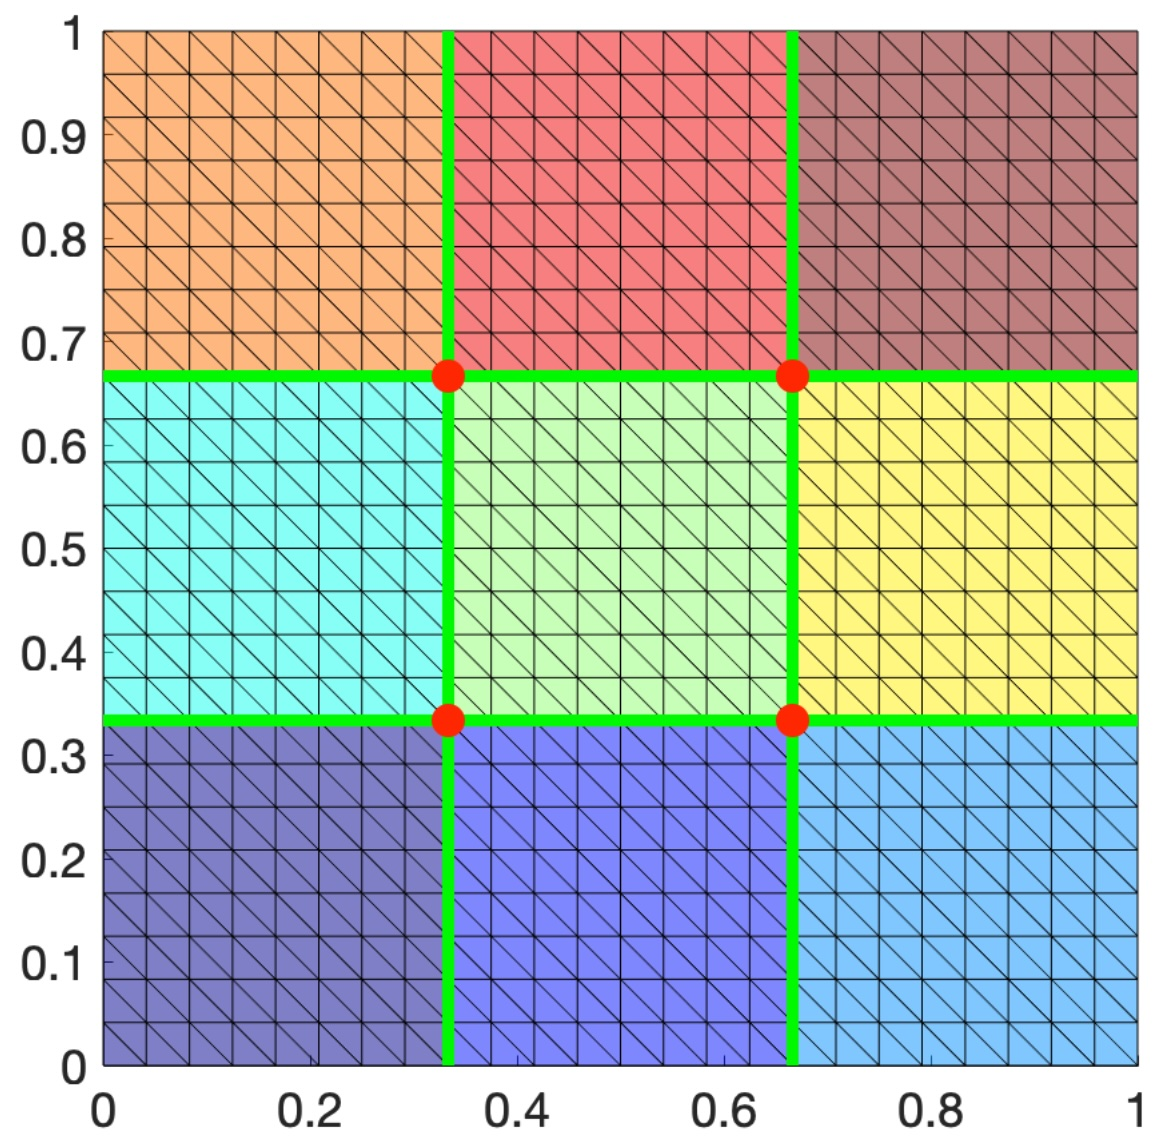
\includegraphics[width=0.45\textwidth]{images/decomposed_domain.jpg}
				\end{figure}
			\end{column}
            \hspace*{-20mm}
			\begin{column}{0.4\textwidth}
				\vspace*{-9mm}
				\begin{figure}
					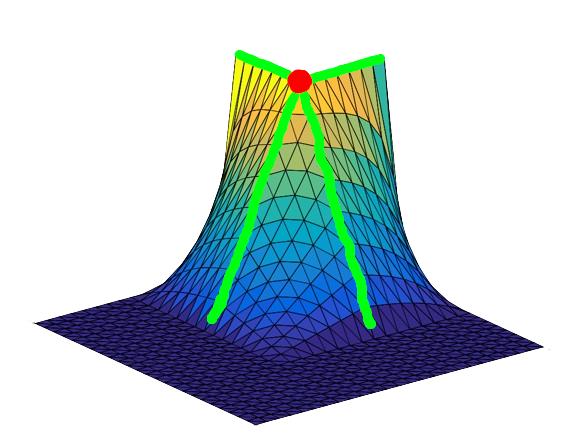
\includegraphics[width=0.65\textwidth]{images/r22.png}
				\end{figure}
			\end{column}
		\end{columns}
	}
	\only<3>{
		Summary:
		\begin{equation*}
			\Phi =
			\begin{pmatrix}
				\Phi_I \\  \Phi_\Gamma
			\end{pmatrix} =
			\begin{pmatrix}
				-A_{II}^{-1}A_{I\Gamma}\Phi_\Gamma \\ \Phi_\Gamma
			\end{pmatrix}
		\end{equation*}
		and
		\begin{equation*}
			P_0 \coloneqq \Phi\text{,}\quad R_0 \coloneqq \Phi^T
		\end{equation*}
	}
\footnotetext{\tiny Dohrmann, Widlund (2017)}
\end{frame}

\begin{frame}[noframenumbering]{Motivation: linear vs nonlinear preconditioning}
	Discretized nonlinear partial differential equation: $F(u) = 0$
	\begin{columns}
		\begin{column}{0.5\textwidth}
			\vspace*{-4mm}
			\begin{block}{\normalsize Linear preconditioner}
				\begin{enumerate}
					\item Linearize:
					      \begin{equation*}
						      DF(u^k)\delta^{k+1} = F(u^k)
					      \end{equation*}
					\item Improve linear solver performance with Schwarz preconditioner:
					      \begin{equation*}
						      \mathcal{M}_{OS}^{-1}DF(u^k)\delta^{k+1} = \mathcal{M}_{OS}^{-1}F(u^k)
					      \end{equation*}
				\end{enumerate}
				\vspace*{4mm}
				Goal:
				\begin{itemize}
					\item $\kappa(\mathcal{M}_{OS}^{-1}DF(u^k)) \approx 1$
				\end{itemize}
			\end{block}
		\end{column}
		\begin{column}{0.5\textwidth}
			\vspace*{-4mm}
			\begin{block}{\normalsize Nonlinear preconditioner}
				\begin{enumerate}
					\item Reformulate the original nonlinear problem based on local nonlinear corrections
					      \begin{equation}
						      \mathcal{F}(u) = G(F(u)) = 0
					      \end{equation}
					\item Linearize $\mathcal{F}(u) = 0$ and solve iterativily
				\end{enumerate}
				Goal:
				\begin{itemize}
					\item $\mathcal{F}(u)$ more linear than $F(u)$
					\item $\mathcal{F}(u^*) = 0 \iff F(u^*) = 0$
				\end{itemize}
			\end{block}
		\end{column}
	\end{columns}

\end{frame}

\begin{frame}[noframenumbering]{One-level nonlinear Schwarz}
	\note{This requires two levels of Newton's method. Seems to be less efficient at first glance. The advantage of this method becomes apparent when solving problems with local regions of highly nonlinear behavior e.g. laminar flow with localized turbulence\\}
	\note{The algorithm shows how this method is essentially the same as applying Newton directly, but to the function $\mathcal{F}$ instead of $F$.\\}
	\note{Constructin $A$ requires inversion of all the local matrices. The result of this is that the linear system is already preconditioned. Note that the preconditioner can not be changed on the fly. It results directly from the nonlinear problem}
	\begin{columns}
		\begin{column}{0.53\textwidth}
			\begin{algorithm}[H]
				\small
				\begin{algorithmic}[1]
					\State $k\gets0$
					\State \textbf{Init.} $u^k$
					\State \textbf{Eval.} $F(u^k)$
					\While{stop. cond. false}
					\State \textbf{Eval.} $\mathcal{F}_1(u^k)$
					\State \textbf{Eval.} $D\mathcal{F}_1(u^k)$
					\State \textbf{Solve} (e.g. GMRES) $D\mathcal{F}_1(u^k)\delta^k = \mathcal{F}_1(u^k)$
					\State \textbf{Update} $u^{k+1} = u^k - \delta^k$
					\State $k\gets k+1$
					\State \textbf{Eval.} $F(u^k)$
					\EndWhile
				\end{algorithmic}
				\caption*{\small Nonlinear Schwarz}
			\end{algorithm}
		\end{column}
		\begin{column}{0.47\textwidth}
			\begin{algorithm}[H]
				\small
				\begin{algorithmic}[1]
					\State $k \gets 0$
					\State \textbf{Init.} $g_i^k$
					\State \textbf{Eval.} $F_i^k\coloneqq R_iF(u-P_ig_i^k)$
					\While{stop. cond. false}
					\State \textbf{Eval.} $DF_i^k= R_iDF(u-P_ig_i^k)P_i$
					\State \textbf{Solve} (direct) $DF_i^k\delta^k = F_i^k$
					\State \textbf{Update} $g_i^{k+1} = g_i^k + \delta^k$
					\State $k\gets k+1$
					\State \textbf{Eval.} $F_i^k\coloneqq R_iF(u-P_ig_i^k)$
					\EndWhile
					\State $g_i\gets g_i^k$
				\end{algorithmic}
				\caption*{\small Evaluation of $g_i\coloneqq T_i(u)$}
			\end{algorithm}
		\end{column}
	\end{columns}
\end{frame}

\begin{frame}[noframenumbering]{Nonlinear Schwarz domain decomposition methods}% \footnote{\tiny Cai and Keyes 2002} \footnote{\tiny Dolean, Gander, Cherie, Kwok and Masson 2016}}
	\vspace{-5mm}
	\begin{columns}
		\begin{column}{0.7\textwidth}
      \centering
			\begin{block}{\normalsize Alternative nonlinear problem}
				The discretized nonlinear partial differential equation
				\begin{equation*}
					F(u) = 0,\, F : V\mapsto V
				\end{equation*}
				is reformulated to
				\begin{equation*}
          \mathcal{F}(u) = 0,\, \mathcal{F} : V\mapsto V.
				\end{equation*}
				The new nonlinear function $\mathcal{F}(u)$ is given implicitly by computing local nonlinear corrections $T_i(u),\,i = 1,\dots,N$ on (overlapping) subdomains
			\end{block}
		\end{column}
		\begin{column}{0.3\textwidth}
			\begin{figure}
				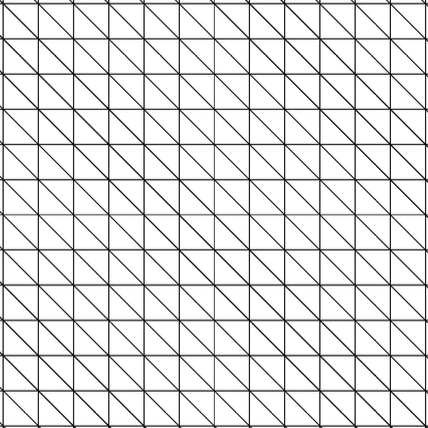
\includegraphics[height=0.4\textwidth,width=0.7\textwidth]{images/DD-mesh-1.png}
				\vspace{-2mm}
				\caption{\tiny Global domain $\Omega$, FE space $V$}
			\end{figure}
			\vspace{-6mm}
			\begin{figure}
				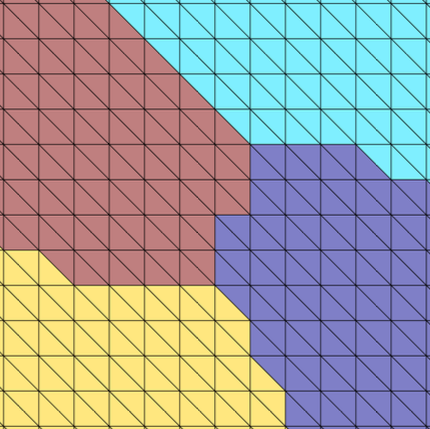
\includegraphics[height=0.4\textwidth,width=0.7\textwidth]{images/DD-mesh-2.png}
				\vspace{-2mm}
				\caption{\tiny Subdomains $\Omega_i$, FE spaces $V(\Omega_i)$}
			\end{figure}
			\vspace{-6mm}
			\begin{figure}
				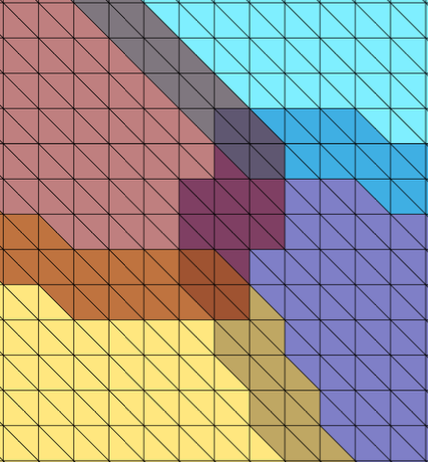
\includegraphics[height=0.4\textwidth,width=0.7\textwidth]{images/DD-mesh-3.png}
				\vspace{-2mm}
				\caption{\tiny Overlapping SDs $\Omega_i'$, FE spaces $V_i$}
			\end{figure}
		\end{column}

	\end{columns}
\end{frame}

\begin{frame}[noframenumbering]{Adding a coarse level \footnote{\tiny Toselli, Widlund (2005)}}

	{\Large Linear Schwarz preconditioners}
	\vspace*{4mm}
	\begin{columns}
		\begin{column}{0.5\textwidth}
			{\bf One-level Schwarz preconditioner}
			\begin{equation*}
				\mathcal{M}^{-1}_{OS-1}=\sum_{i=1}^{N}P_i(R_iAP_i)^{-1}R_i
			\end{equation*}
			\begin{block}{\normalsize Condition number estimate:}
				\begin{equation*}
					\kappa(\mathcal{M}^{-1}_{OS-1}A)\leq C(1+\frac{1}{H\delta})
				\end{equation*}
			\end{block}
		\end{column}
		\begin{column}{0.5\textwidth}
			{\bf Two-level Schwarz preconditioner}
			\vspace*{3mm}
			\begin{equation*}
				\mathcal{M}^{-1}_{OS-2}=P_0(R_0AP_0)^{-1}R_0 + \mathcal{M}^{-1}_{OS-1}
			\end{equation*}
			\begin{block}{\normalsize Condition number estimate:}
				\begin{equation*}
					\kappa(\mathcal{M}^{-1}_{OS-2}A)\leq C(1+\frac{H}{\delta})
				\end{equation*}
			\end{block}
		\end{column}
	\end{columns}
	\vspace*{4mm}
	\centering
	with subdomain size $H$ and overlap width $\delta$
	% \let\thefootnote\relax\footnote{Dohrmann, Widlund 2012}
\end{frame}


\begin{frame}[noframenumbering]{LDC coarse basis functions}
	\begin{figure}
		\centering
		\begin{subfigure}{0.5\textwidth}
			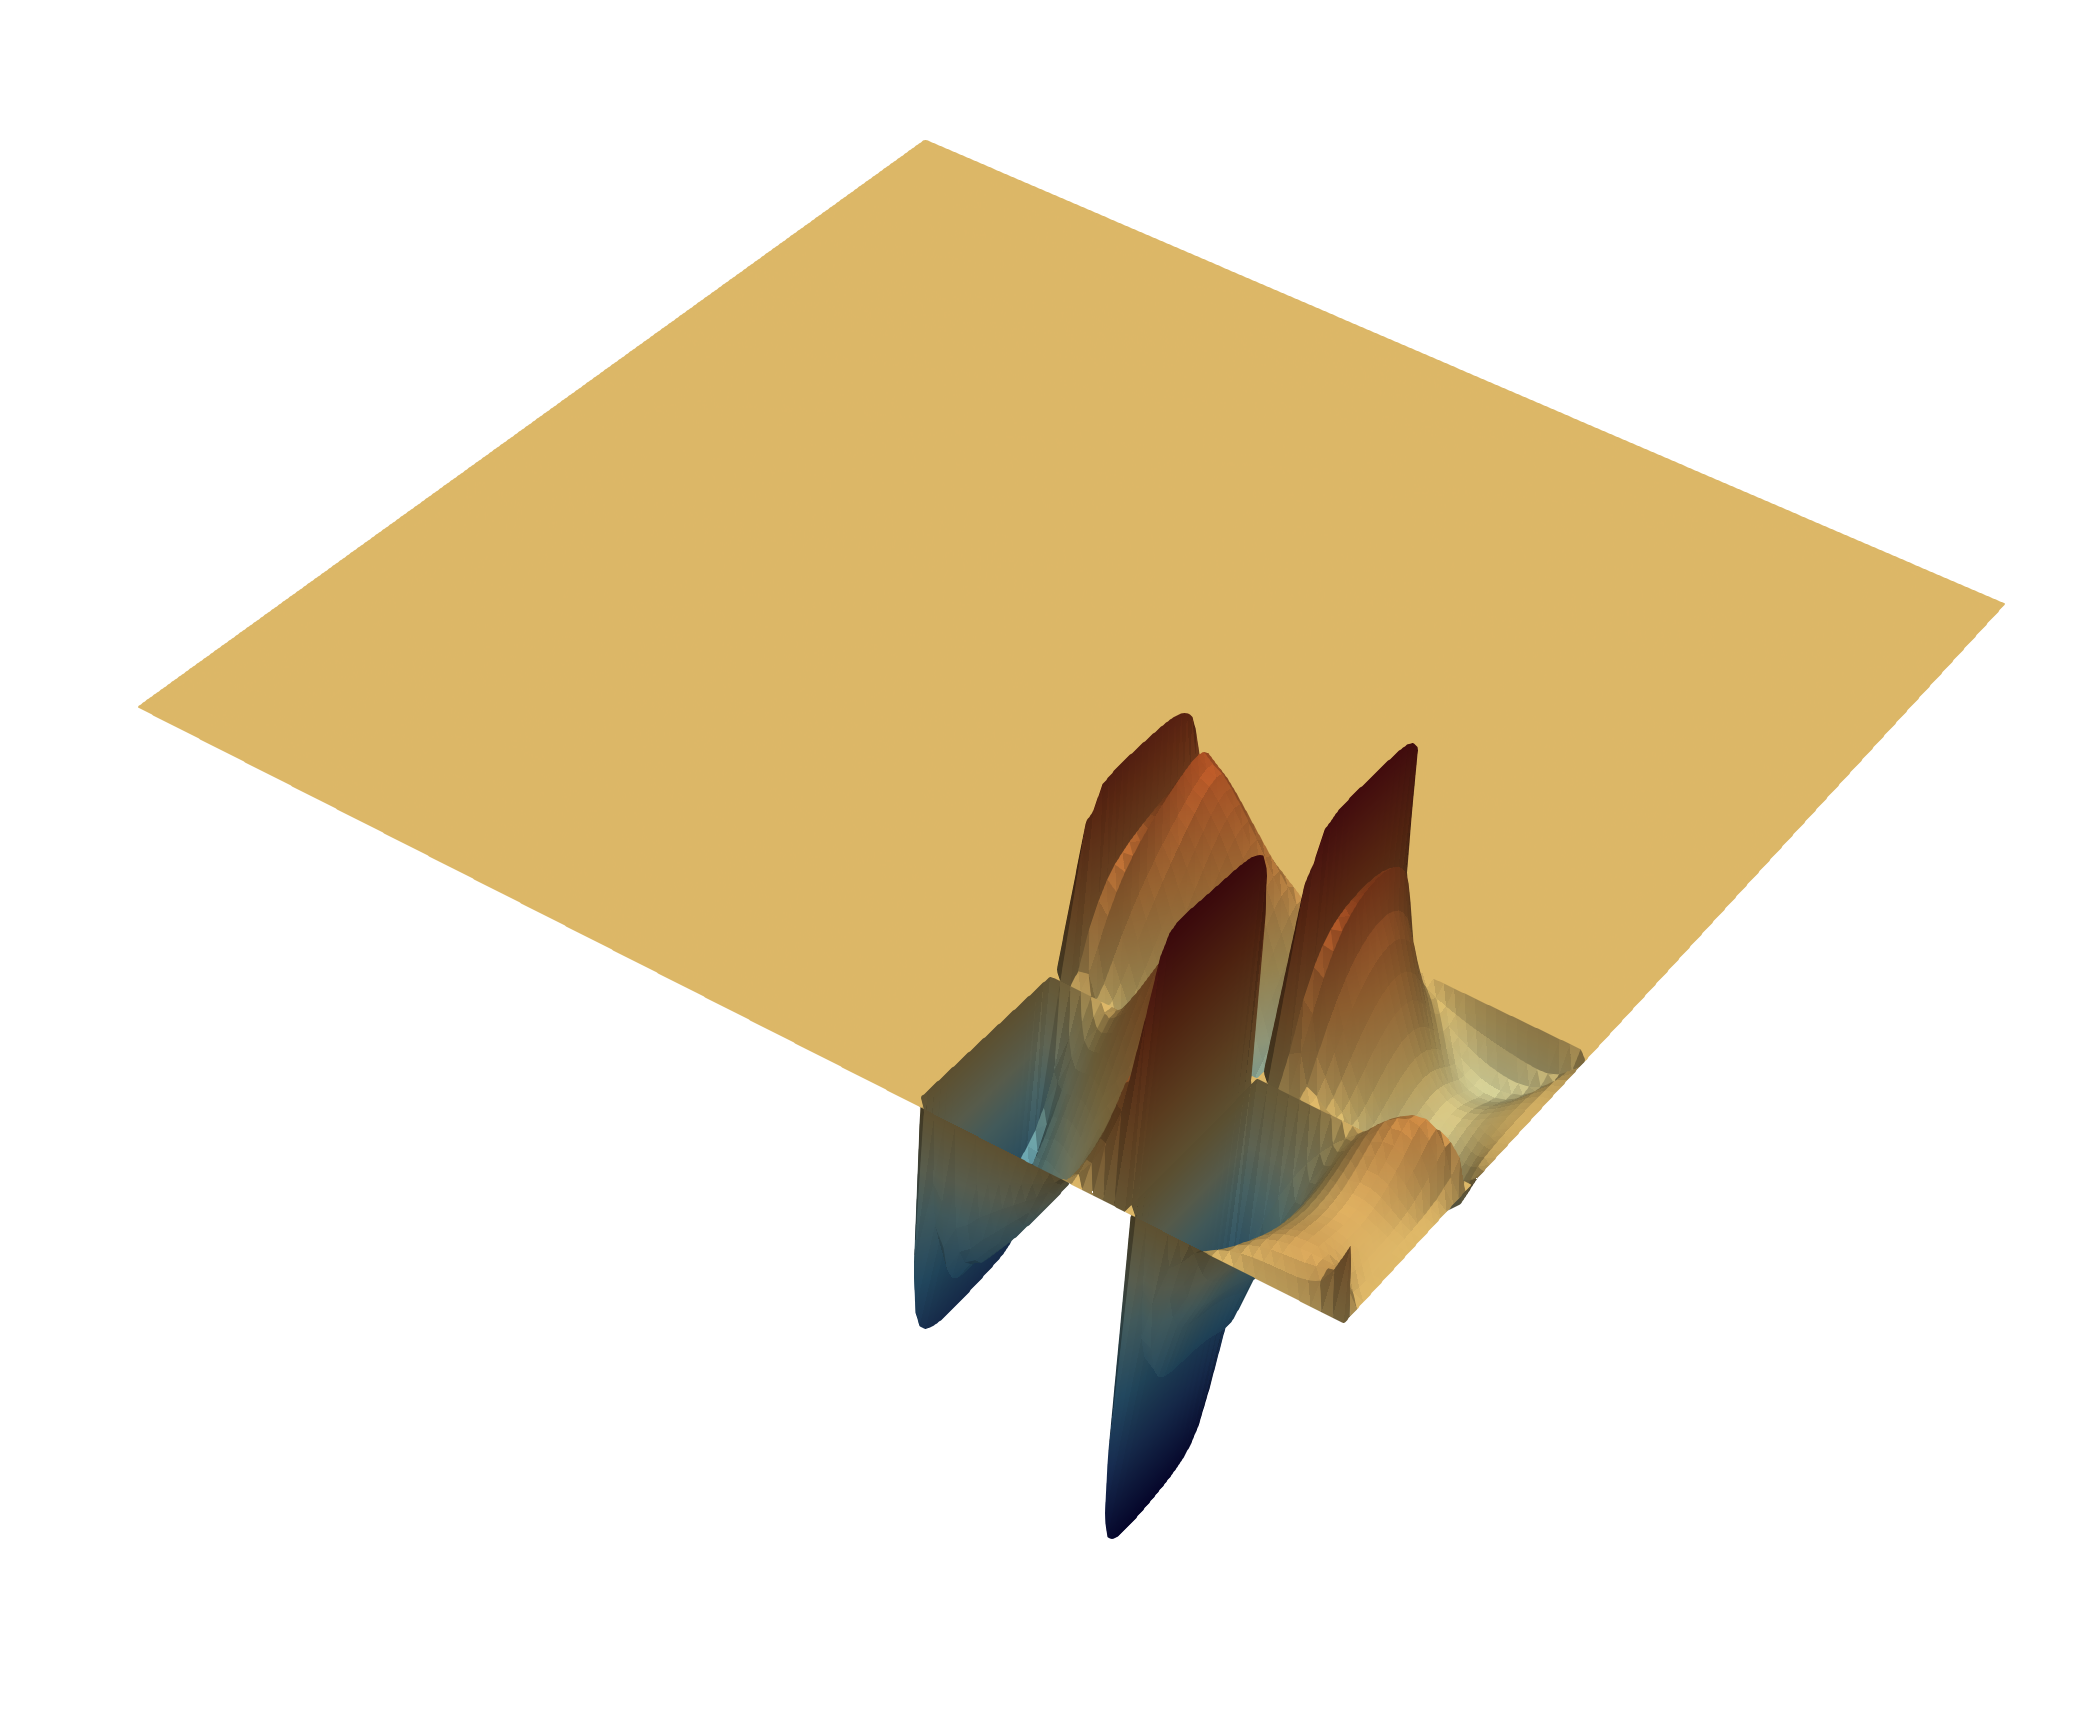
\includegraphics[width=\textwidth]{images/RGDSW-y}
			\caption{RGDSW $y$ component.}
		\end{subfigure}%
		\begin{subfigure}{0.5\textwidth}
			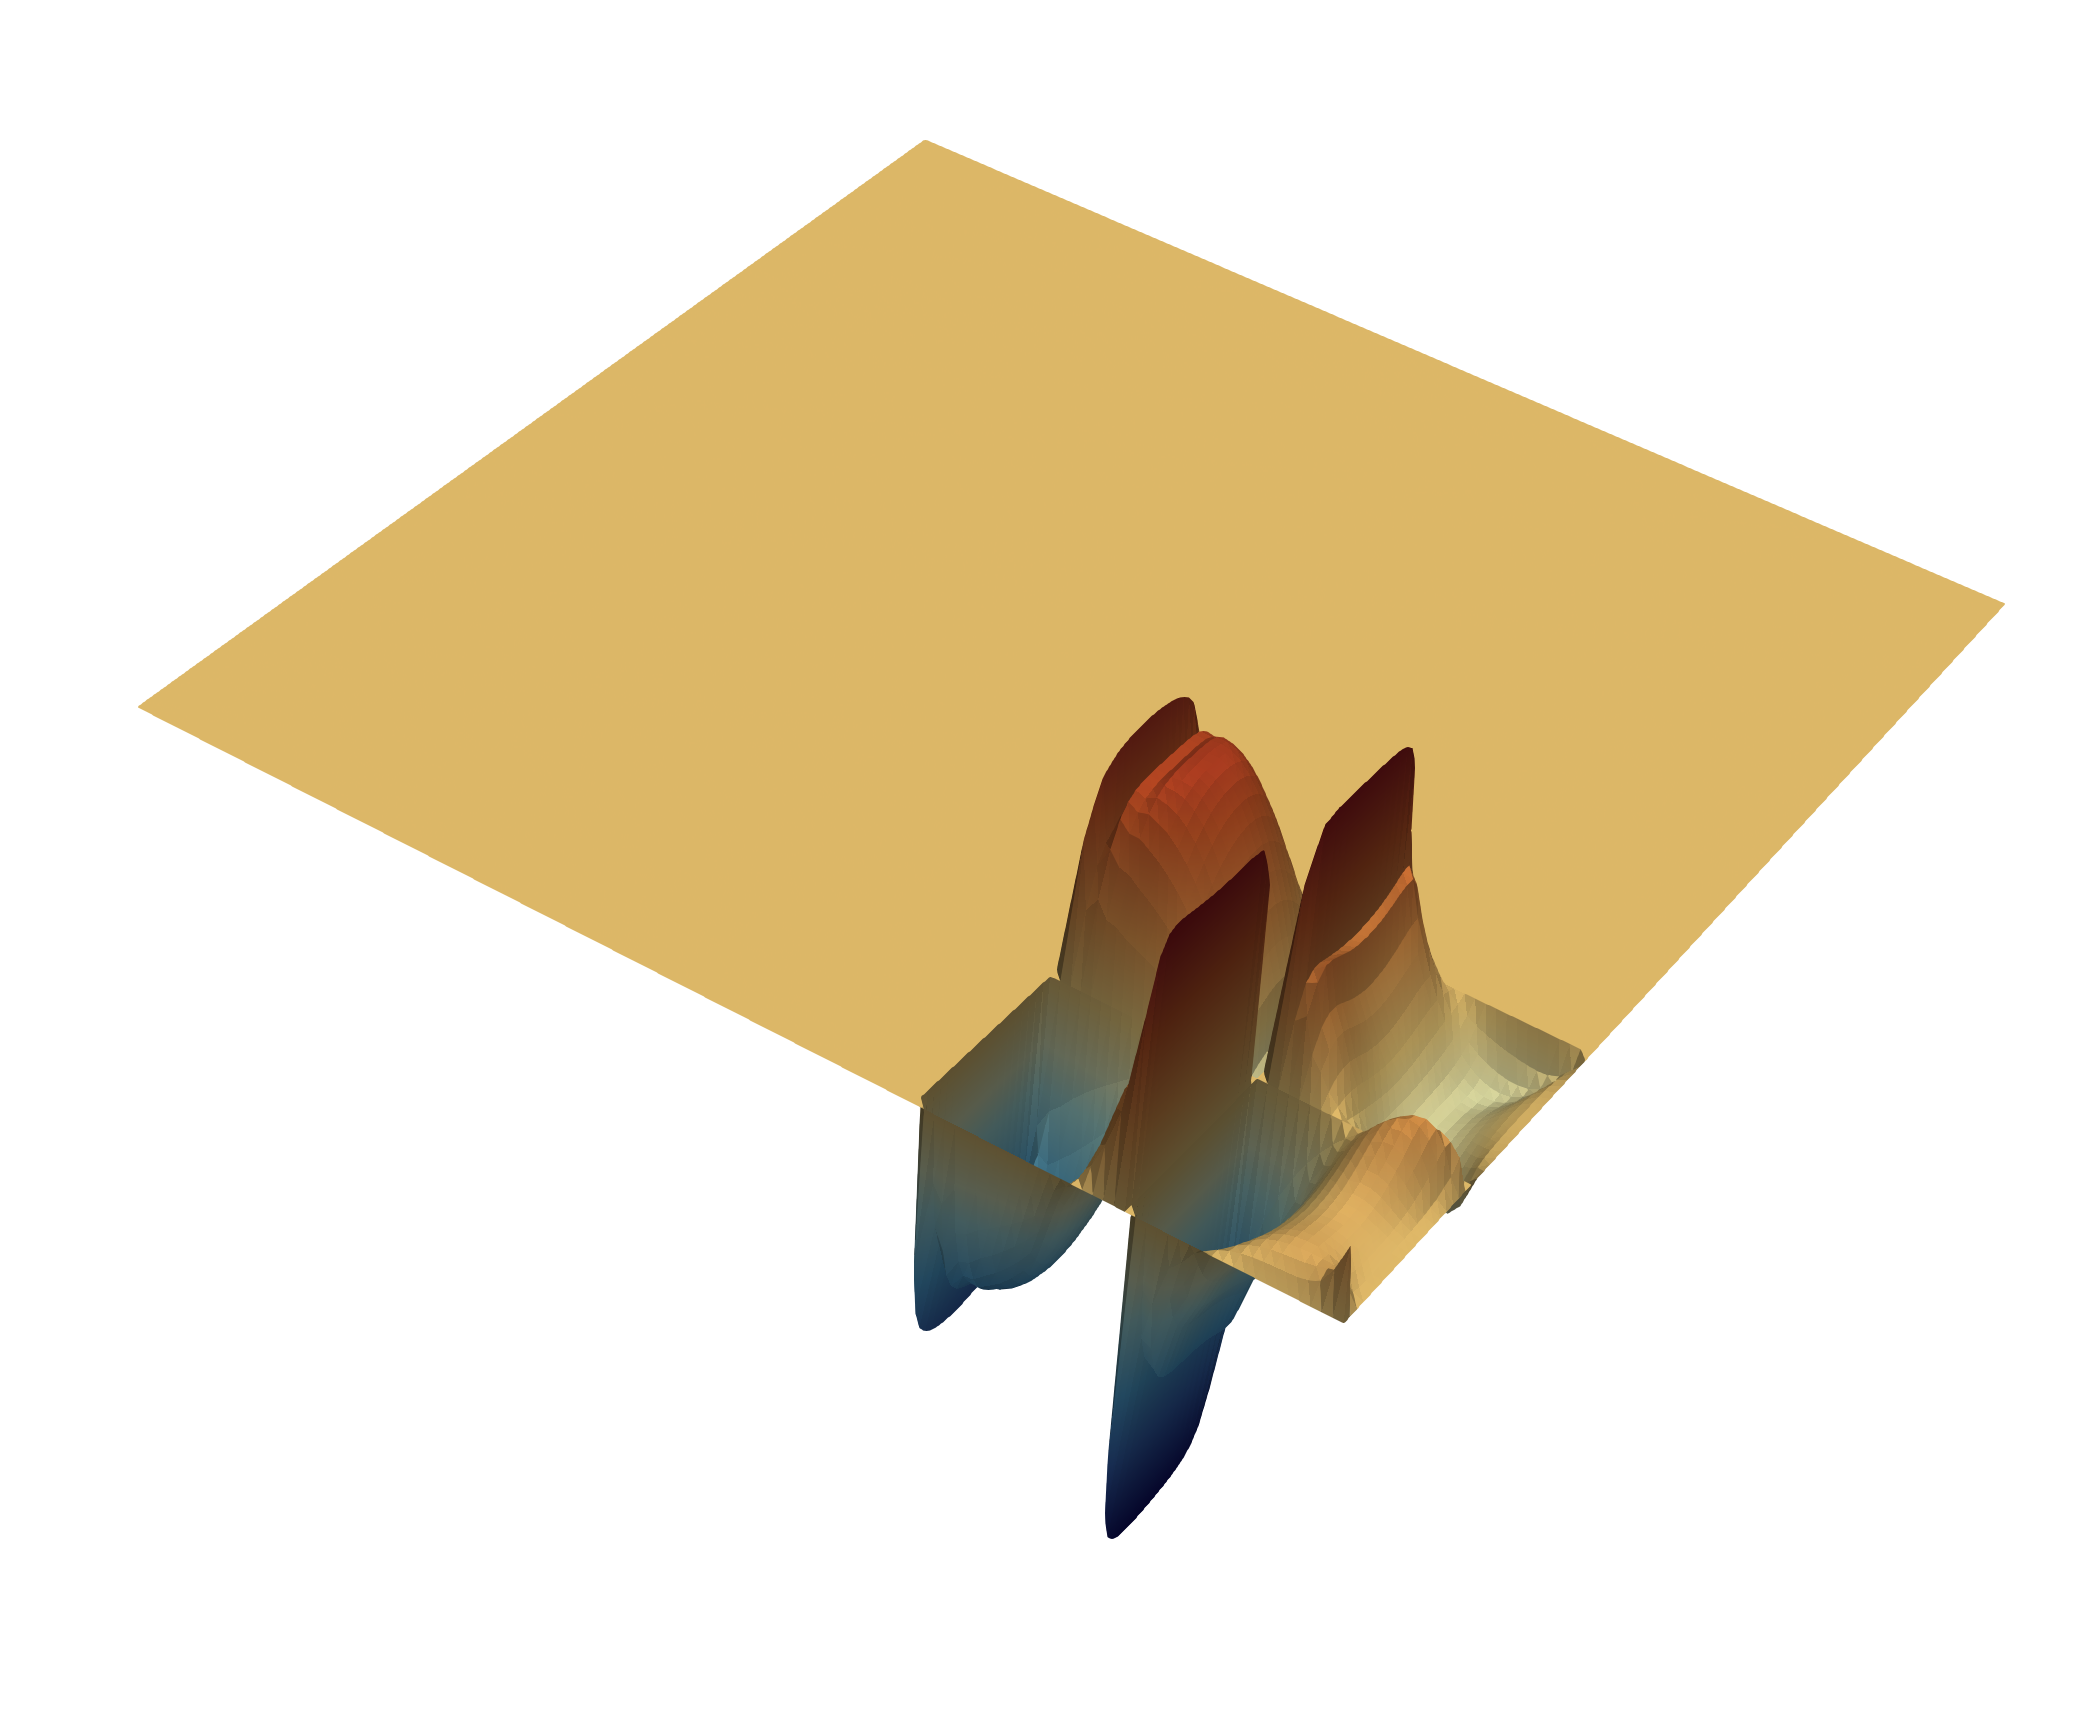
\includegraphics[width=\textwidth]{images/MsFEM-y}
			\caption{MsFEM $y$ component.}
		\end{subfigure}
		\caption{Components of $x$ velocity coarse basis function.}
	\end{figure}
\end{frame}

\begin{frame}[noframenumbering]{2D compressible plane-stress neo-Hookean material}
	\vspace{0mm}
	\begin{columns}
		\begin{column}{0.4\textwidth}%
			\begin{align*}
				\label{eq:nonlinelas}
				\begin{split}
					-\mathrm{div}(P(F)) = f_{vol}\; & \mathrm{in}\;\Omega,           \\
					u = g_D \;                      & \mathrm{on}\;\partial\Omega_D, \\
					n\cdot P(F) = g_N\;             & \mathrm{on}\;\partial\Omega_N,
				\end{split}
			\end{align*}
			\begin{figure}
				\centering
				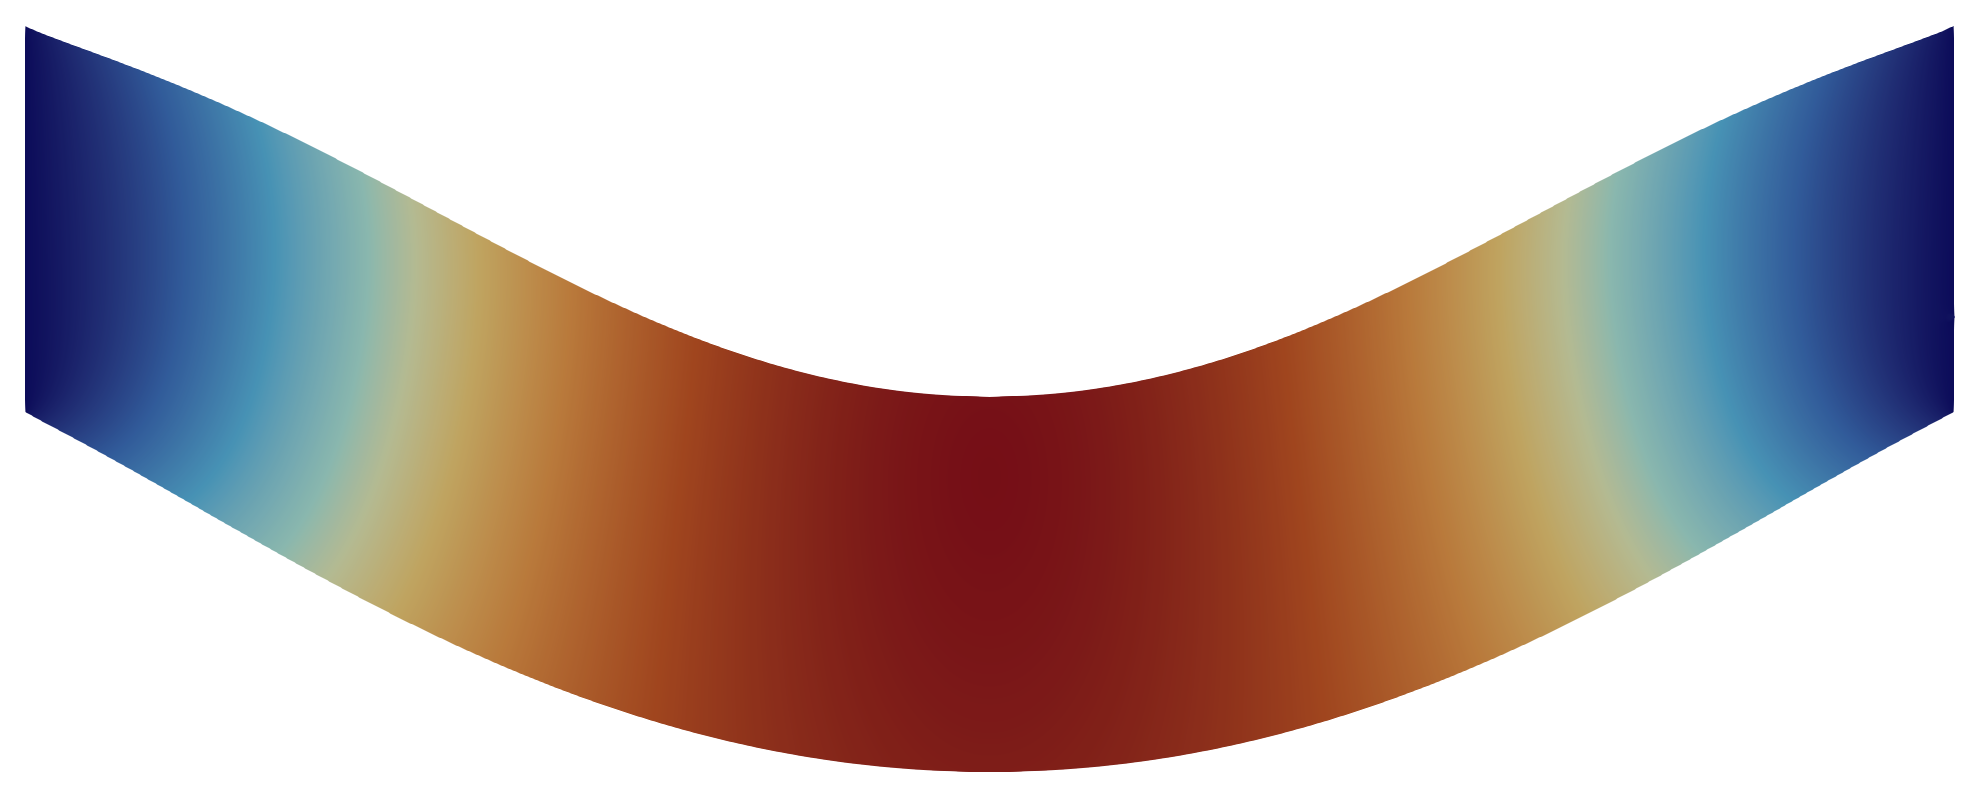
\includegraphics[width=0.9\textwidth]{images/beam2D.png}
				\caption{2D beam with applied volume force.}
				\label{fig:beam2d}
			\end{figure}
		\end{column}%
		\begin{column}{0.6\textwidth}
			\vspace{-1em}
			\centering
			\begin{itemize}
				% \setlength{\itemsep}{15pt}
				\item $F$ Deformation gradient
				\item $P(F) = \frac{E}{1(1+\nu)}(F-F^{-T}) + \frac{E\nu}{(1+\nu)(1-2\nu)}\mathrm{ln}(\mathrm{det}(F)F^{-T})$
				\item $\nu$ = 0.3
				\item $E$ = 210 GPa
				\item $5\textrm{m}\times 1\textrm{m}$ 2D mesh with \numgru{2572710} nodes
        \item $g_D = 0$ on short edges
				\item $g_N = 0$ on long edges
				\item P1 elements
        \item Solver relative tolerance: $10^{-4}$
        \item MsFEM coarse space \footnotemark{}
				% \item $f_{vol} = (0,-f_y)$
			\end{itemize}
		\end{column}
	\end{columns}
  \footnotetext{\tiny Dohrmann, Widlund (2017)}
\end{frame}

\begin{frame}[noframenumbering]{Strong scaling: nonlinear elasticity}
	\begin{itemize}
		\item $f_y = 4$ MN/m$^{2}$
	\end{itemize}
	\begin{figure}
		\centering
		\begin{tikzpicture}
	\pgfplotsset{
		every axis/.append style={
				ybar stacked,
				width=13cm,
				height=7cm,
				ylabel={Runtime (seconds)},
				xlabel={Num. subdomains},
				symbolic x coords={72, 144, 288, 576, 1152},
				xtick=data,
				enlarge x limits=0.15,
				legend style={at={(1,1)},anchor=north east},
				axis lines*=left, ymajorgrids, yminorgrids,
				ymin=0,
				ymax=100,
				bar width=8pt,
				minor y tick num=1,
				xticklabel style={rotate=0,xshift=0ex,anchor=north},
				cycle list name=Set2-5,
			},
		% Ensures that bars are plotted full
		every axis plot/.append style={
				fill,
			},
	}
	\tikzstyle{mynodestyle} = [rotate=90, anchor=west]

	% Solver = H1
	\begin{axis}[bar shift=11pt, hide axis]
		% Another option for relative node placement
		% \node [left=11pt of 256.base, anchor=base] {test}; % Custom number above bar for 256
		\node[mynodestyle] at ([xshift=11pt]axis cs:72,58) {$65$ $(3)$};
		\node[mynodestyle] (one) at ([xshift=11pt]axis cs:144,27.5) {$62$ $(3)$};
		\node[mynodestyle] at ([xshift=11pt]axis cs:288,13.6){$53$ $(3)$};
		\node[mynodestyle] at ([xshift=11pt]axis cs:576,6.8){$44$ $(3)$};
		\node[mynodestyle] at ([xshift=11pt]axis cs:1152,4.5){$41$ $(3)$};
		\node [mynodestyle](oneRe) at ([xshift=11pt]axis cs:72,1) {H};

		\addplot coordinates {(72,58) (144,27.5) (288,13.6) (576,6.8) (1152,4.5)};
	\end{axis}

	% Solver = Add.
	\begin{axis}[bar shift=0pt, hide axis]
		\node[mynodestyle] at (axis cs:72,81.2) {$100$ $(4)$};
		\node[mynodestyle](two) at (axis cs:144,34.5) {$97$ $(4)$};
		\node[mynodestyle]at (axis cs:288,17) {$81$ $(4)$};
		\node[mynodestyle]at (axis cs:576,9) {$75$ $(4)$};
		\node[mynodestyle]at (axis cs:1152,6.2) {$71$ $(4)$};
		\node [mynodestyle]at (axis cs:72,1) {Add.};

		\addplot+ coordinates {(72,81.2) (144,34.5) (288,16.9) (576,9) (1152,6.2)};
	\end{axis}

	% Solver = NKS

	\begin{axis}[bar shift=-11pt]
		%% Overlap = 10
		% \node [mynodestyle] at([xshift=-11pt]axis cs:72,42) {$190$ $(5)$};
		% \node [mynodestyle](three) at([xshift=-11pt]axis cs:144,22.5) {$200$ $(5)$};
		% \node [mynodestyle]at([xshift=-11pt]axis cs:288,11.8) {$170$ $(5)$};
		% \node [mynodestyle]at([xshift=-11pt]axis cs:576,7.3) {$150$ $(5)$};
		% \node [mynodestyle]at([xshift=-11pt]axis cs:1152,5.2) {$135$ $(5)$};
		% \node [mynodestyle]at ([xshift=-11pt]axis cs:72,1) {NKS};
		%
		% \addplot+ coordinates {(72,41.7) (144,22.5) (288,11.8) (576,7.3) (1152,5.2)};


		%% Overlap = 5
		\node [mynodestyle]at([xshift=-11pt]axis cs:72,33) {$162$ $(5)$};
		\node [mynodestyle](three) at([xshift=-11pt]axis cs:144,16) {$159$ $(5)$};
		\node [mynodestyle]at([xshift=-11pt]axis cs:288,8) {$136$ $(5)$};
		\node [mynodestyle]at([xshift=-11pt]axis cs:576,4) {$124$ $(5)$};
		\node [mynodestyle]at([xshift=-11pt]axis cs:1152,3.2) {$108$ $(5)$};
		\node [mynodestyle]at([xshift=-11pt]axis cs:72,1) {NKS};

		\addplot+ coordinates {(72,34) (144,17.1) (288,9.1) (576,5.1) (1152,4.2)};
		\node[text width=1.6cm] (gmres) at (axis cs:144,80){GMRES its. (Newton its.)};

	\end{axis}

	\draw [thin] (gmres) --  (one);
	\draw [thin] (gmres) --  (two);
	\draw [thin] (gmres) --  (three);

\end{tikzpicture}

		\label{fig:strong-scalability-elascticity}
	\end{figure}
\end{frame}

\begin{frame}[noframenumbering]{Newton-Krylov-Schwarz vs nonlinear Schwarz}
	\begin{itemize}
		\item $576$ Subdomains
	\end{itemize}
	\begin{figure}
		\centering
		\begin{tikzpicture}
	\pgfplotsset{
		every axis/.append style={
				legend style={at={(1,1)},anchor=north east},
				axis lines*=left, ymajorgrids, yminorgrids,
				width=13.8cm, height=7cm,
				ymin=0,
				ymax=13,
				ybar stacked,
				bar width=8pt,
				minor y tick num=1,
				symbolic x coords={1,2,3,4,5,6},
				xtick={1,2,3,4,5,6},
				xticklabels from table={\hybrid}{Force},
				xticklabel style={rotate=0,xshift=0ex,anchor=north},
				ylabel={Runtime (seconds)},
				xlabel={Force in MN/m$^{2}$},
				cycle list name=Set2-5,
			},
		every axis plot/.append style={fill},
	}

	\tikzstyle{mynodestyle} = [rotate=90, anchor=west]

	\pgfplotstableread{
		Location Force  GlobalSolve   InnerSolve   CoarseSolve   GMRES    Other
		1        4      6.9           2.73         2.2           0.58     1.39
		2        4.5    7.3           3.2          2.1           0.59     1.41
		3        5      6.8           2.7          2.2           0.57     1.33
		4        6      7.1           2.9          2.2           0.61     1.39
		5        7      7.3           3            2.3           0.61     1.39
		6        7.5    0             0            0             0        0
	}\hybrid

	\pgfplotstableread{
		Location Force  GlobalSolve   InnerSolve   CoarseSolve   GMRES    Other
		1        4      9.1           3.38         3             0.96     1.76
		2        4.5    9.1           3.4          2.85          1        1.85
		3        5      9.2           3.5          3             1        1.7
		4        6      9.2           3.6          2.8           1        1.8
		5        7      0             0            0             0        0
		6        7.5    0             0            0             0        0
	}\RGDSWtwo
 
  %% Overlap = 10
	% \pgfplotstableread{
	% 	Location Force  GlobalSolve   GMRES    Other
	% 	1        4      7.2           6.5      0.7
	% 	2        4.5    8.2           7.4      0.8
	% 	3        5      0             0        0
	% 	4        6      0             0        0
	% 	5        7      0             0        0
	% 	6        7.5    0             0        0
	% }\NKS

  %% Overlap = 5
	\pgfplotstableread{
		Location Force  GlobalSolve   GMRES    Other
		1        4      5.1           4.4      0.7
		2        4.5    6.1           5.2      0.9
		3        5      0             0        0
		4        6      0             0        0
		5        7      0             0        0
		6        7.5    0             0        0
	}\NKS

	\begin{axis}[bar shift=0pt, hide axis]
		\node[mynodestyle]at (axis cs:1,0) {Add.};
		\node[mynodestyle] (two) at (axis cs:1,9.1) {$75$ $(4)$};
		\node[mynodestyle] at(axis cs:2,9.1) {$76$ $(4)$};
		\node[mynodestyle] at(axis cs:3,9.1) {$76$ $(4)$};
		\node[mynodestyle] at(axis cs:4,9.1) {$76$ $(4)$};
		\node at(axis cs:5,.4) {\scriptsize\color{red}\ding{55}};
		\node at(axis cs:6,.4) {\scriptsize\color{red}\ding{55}};

		\addplot+ table [x=Location, y=InnerSolve] {\RGDSWtwo};
		\addplot+ table [x=Location, y=CoarseSolve] {\RGDSWtwo};
		\addplot+ table [x=Location, y=GMRES] {\RGDSWtwo};
		\addplot+ table [x=Location, y=Other] {\RGDSWtwo};
	\end{axis}

	\begin{axis}[bar shift=11pt]
		\node[mynodestyle] at ([xshift=11pt]axis cs:1,0) {H};
		\node[xshift=11pt,mynodestyle] (three) at (axis cs:1,6.9) {$44$ $(3)$};
		\node[xshift=11pt,mynodestyle] at (axis cs:2,7.3) {$44$ $(3)$};
		\node[xshift=11pt,mynodestyle] at (axis cs:3,6.8) {$44$ $(3)$};
		\node[xshift=11pt,mynodestyle] at (axis cs:4,7.1) {$45$ $(3)$};
		\node[xshift=11pt,mynodestyle] at (axis cs:5,7.3) {$47$ $(3)$};
		\node[xshift=11pt,rotate=0] at  (axis cs:6,.4) {\scriptsize\color{red}\ding{55}};

		\addplot+ table [y=InnerSolve] {\hybrid}; \addlegendentry{Inner solve}
		\addplot+ table [y=CoarseSolve] {\hybrid}; \addlegendentry{Coarse solve}
		\addplot+ table [y=GMRES] {\hybrid}; \addlegendentry{GMRES}
		\addplot+ table [y=Other] {\hybrid}; \addlegendentry{Other}
	\end{axis}

	\begin{axis}[bar shift=-11pt, hide axis, cycle list shift=2]
		\node[mynodestyle]at ([xshift=-11pt]axis cs:1,0) {NKS};
		\node[xshift=-11pt,mynodestyle] (one) at (axis cs:1,5.2) {$124$ $(5)$};
		\node[xshift=-11pt,mynodestyle] at (axis cs:2,6.2) {$133$ $(6)$};
		\node[xshift=-11pt,rotate=0] at (axis cs:3,.4) {\scriptsize\color{red}\ding{55}};
		\node[xshift=-11pt,rotate=0] at (axis cs:4,.4) {\scriptsize\color{red}\ding{55}};
		\node[xshift=-11pt,rotate=0] at (axis cs:5,.4) {\scriptsize\color{red}\ding{55}};
		\node[xshift=-11pt,rotate=0] at (axis cs:6,.4) {\scriptsize\color{red}\ding{55}};
		\node[text width=1.5cm] (gmres) at (axis cs:1,12.4) {GMRES its. (Newton its.)};

		\addplot+ table [x=Location, y=GMRES] {\NKS};
		\addplot+ table [x=Location, y=Other] {\NKS};
	\end{axis}

	\draw [thin] (gmres) --  (one);
	\draw [thin] (gmres) --  (two);
	\draw [thin] (gmres) --  (three);

\end{tikzpicture}

		\label{fig:nks-vs-nls}
	\end{figure}
\end{frame}

 \begin{frame}[noframenumbering]{Summary nonlinear elasticity}
   \begin{itemize}
     \item Strong scaling of two-level nonlinear Schwarz variants on-par with NKS
     \item Two-level nonlinear Schwarz variants more robust against nonlinearity
   \end{itemize}
 \end{frame}
%TODO: slides on finding the rgdsw defect and modifying the coarse basis
\begin{frame}[noframenumbering]{Sanity check: nonlinear Laplace}
    \begin{columns}
        \begin{column}{0.47\textwidth}
                \begin{align*}
                    -\nabla\cdot((u^2+1)\nabla u)&=1\quad \text{in}\quad \Omega\subset\mathbb{R}^2,\\
                    u &= 0\quad\text{on}\quad\partial\Omega\\
                    u^0 &= 0
                \end{align*}
                \begin{figure}
                    \centering
                    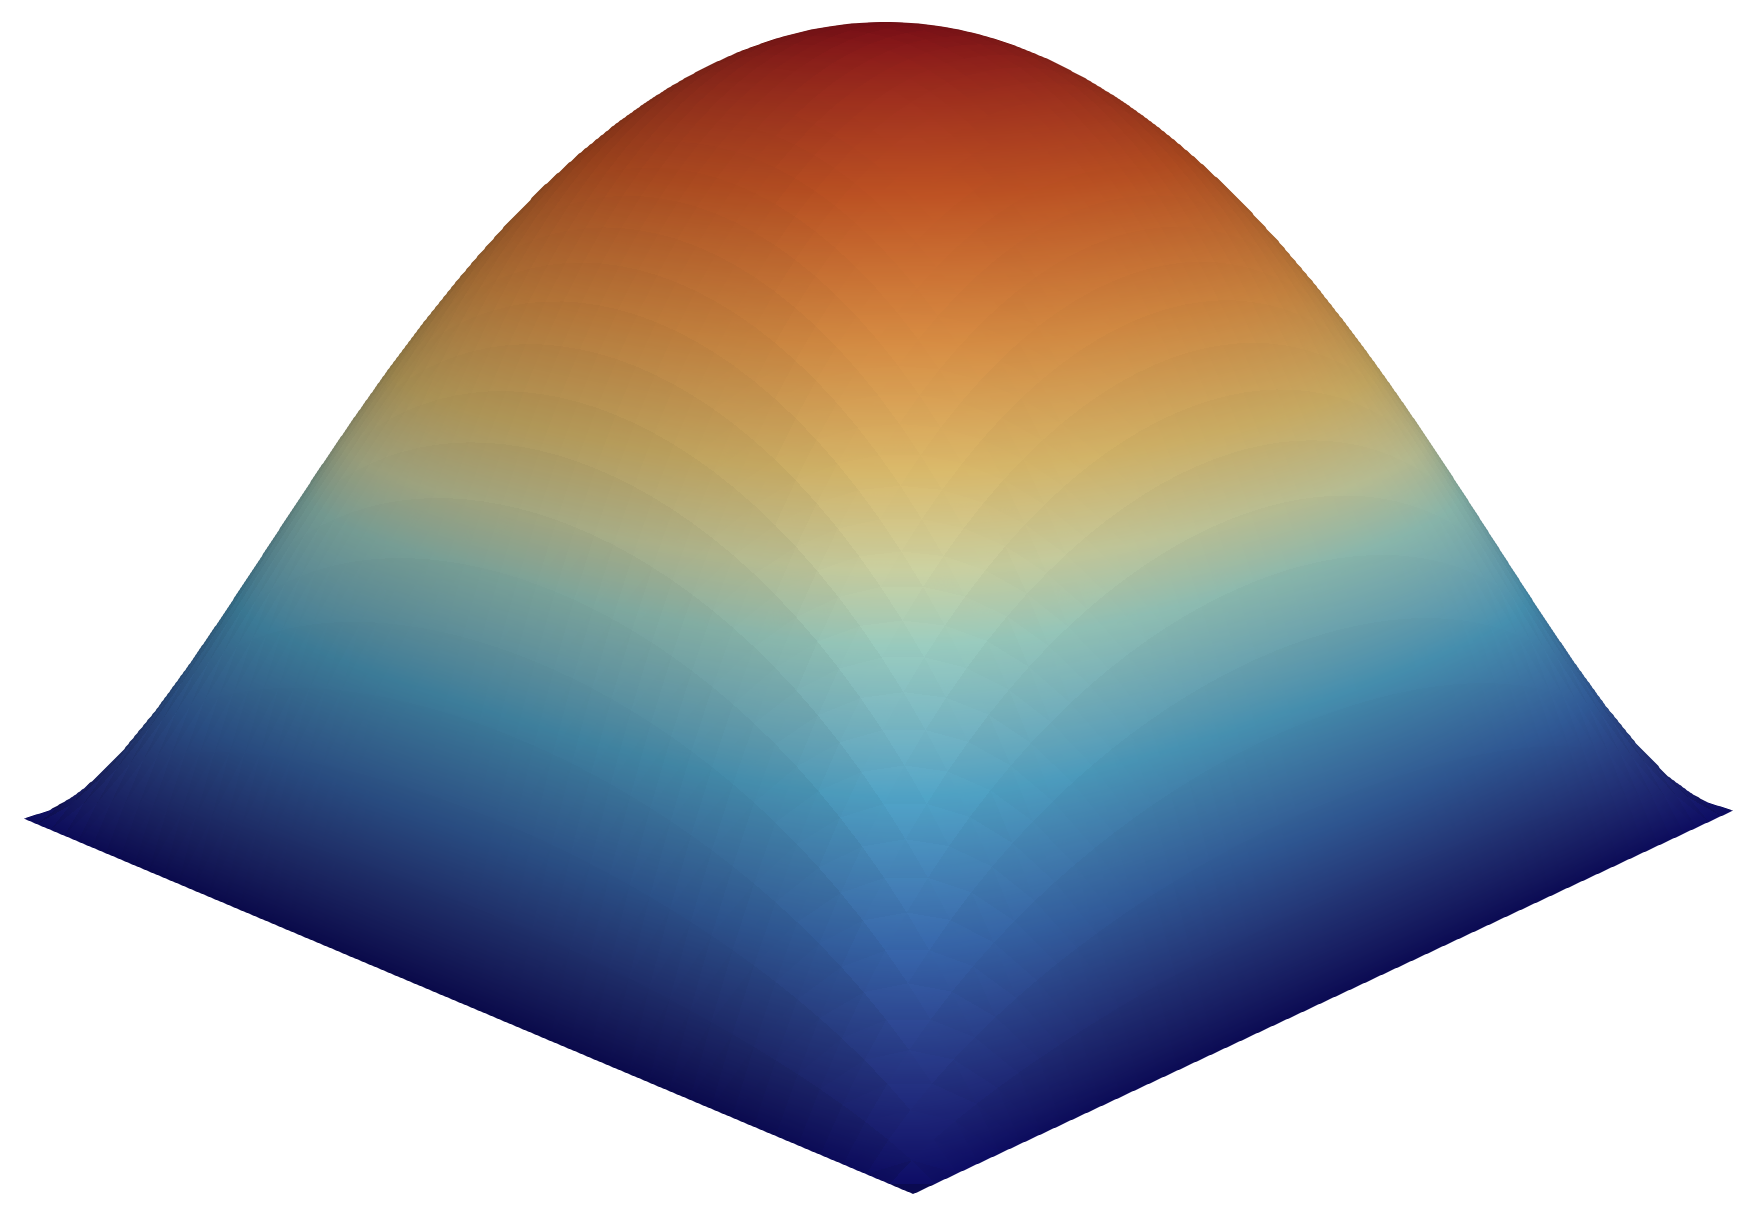
\includegraphics[width=0.45\textwidth]{images/laplace}
                \end{figure}
        \end{column}
        \begin{column}{0.53\textwidth}
               \begin{itemize}
                \setlength{\itemsep}{10pt}
                \item Subdomain size: $300\times300$ elements
                \item Solver relative tolerance: $10^{-4}$
                \item MsFEM coarse space
               \end{itemize} 
        \end{column}
    \end{columns}
 \end{frame}
 
 \begin{frame}[noframenumbering]{Sanity check: weak scalability}
  \begin{figure}
      \centering
      \begin{tikzpicture}
    \pgfplotsset{
      every axis/.append style={
    legend style={at={(0.01,1)},anchor=north west},
    axis lines*=left, ymajorgrids, yminorgrids,
    width=13.8cm, height=7cm,
    ymin=0,
    ymax=455,
    ybar stacked,
    bar width=12pt,
    minor y tick num=1,
    xtick={1,2,3,4,5,6,7},
    % xticklabels={100, 400, 900, 1600, 2500, 3600},
    %xmajorticks=false,
    xticklabels from table={\datatableonelevel}{SubdomainCount},
    xticklabel style={rotate=0,xshift=0ex,anchor=north},
    ylabel={Runtime (seconds)},
    xlabel={Num. subdomains},
      cycle list name=Set2-5,
    },
		every axis plot/.append style={
      fill,
    },
}
\pgfplotstableread{
Location SubdomainCount  GlobalSolve   InnerSolve   CoarseSolve   GMRES   Other
1        100             41.8	         12.6         13.55         5.8     9.85  
2        400	           45.5          12.94        14.0          7.1     11.46 
3        900             47.0          13.15        13.0          8.4     12.45 
4        1600            52.4          14.8         16.65         7.9     13.05 
5        2500            55.1          17.26        15.9          8.2     13.74 
% 6        3600            48.2          13.8         15.12         7.5     11.78 
6        4489            56.02         14           17.4          8.5     16.12 
7        9216            87            14           32.7          22      18.3 
}\datatabletwolevel
\pgfplotstableread{
Location SubdomainCount  GlobalSolve   InnerSolve   CoarseSolve   GMRES    Other
1        100             35.4          10.74        0             18.5     6.16  
2        400             113.6         9.6          0             96.9     7.1   
3        900             171.8         9.7          0             154.7    7.4   
4        1600	           261.2	       14.7		      0             236.3    10.2  
5        2500	           359.4	       18.24        0             328.7    12.46 
% 6        3600	           452.1	       20.9		      0             418.0    13.2  
6        4489            459           24           0             418      17    
7        9216            0             0            0             0        0 
}\datatableonelevel

\begin{axis}[bar shift=-8pt, hide axis]
    \addplot+ table [x=Location, y=InnerSolve] {\datatableonelevel};
    \addplot+ table [x=Location, y=CoarseSolve] {\datatableonelevel};
    \addplot+ table [x=Location, y=GMRES] {\datatableonelevel};
    \addplot+ table [x=Location, y=Other] {\datatableonelevel};
\end{axis}

\begin{axis}[bar shift=8pt]
    \addplot+ table [y=InnerSolve] {\datatabletwolevel}; \addlegendentry{Inner solve}
    \addplot+ table [y=CoarseSolve] {\datatabletwolevel}; \addlegendentry{Coarse solve}
    \addplot+ table [y=GMRES] {\datatabletwolevel}; \addlegendentry{GMRES}
    \addplot+ table [y=Other] {\datatabletwolevel}; \addlegendentry{Other}
\end{axis}
                            
\node[rotate=0] (gmres) at (0.9,1.5) {GMRES its.};
	
\node[rotate=0] (one) at (.7,0.6) {$340$};
\node[rotate=0] (two) at (1.25,0.7) {$120$};

\node[rotate=0] at (2.4,1.5) {$1400$};
\node[rotate=0] at (3.,.75) {$110$};

\node[rotate=0] at (4.1,2.2) {$2000$};
\node[rotate=0] at (4.7,0.75) {$120$};

\node[rotate=0] at (5.8,3.3) {$3000$};
\node[rotate=0] at (6.4,0.8) {$110$};

\node[rotate=0] at (7.5,4.5) {$4000$};
\node[rotate=0] at (8.1,0.8) {$110$};

\node[rotate=0] at (9.2,5.6) {$5000$};
\node[rotate=0] at (9.75,0.8) {$100$};

\node[rotate=0] at (10.9,.2) {\scriptsize\color{red}\ding{55}};
\node[rotate=0] at (11.5,1.2) {$97$};

\draw [arrow] (gmres) --  (one);
\draw [arrow] (gmres) --  (two);


\node[rotate=90] at (0.55,-0.5) {One-lvl.};
\node[rotate=90] at (1.45,-0.5) {Additive};

\end{tikzpicture}


















  \end{figure}
 \end{frame}
